% !TeX root = main.tex

\subsection{Why relative homology?}

The primary tool used in the TCC that we will apply to the analysis of scalar fields is relative persistent homology.
Relative homology provides a powerful representation of a bounded domain that is particularly suited to verifying coverage of a sensor network.
Let $\D$ be a bounded domain with boundary $\B\subset\D$.
For illustrative purposes assume $\D$ is a connected, compact subset of the euclidean plane $\R^2$ so that certain properties of the relative homology of the pair $(\D, \B)$ are known.
Namely, there is exactly one equivalence class in $\hom_2(\D, \B)$, as illustrated in Fig.~\ref{fig:balloons1}.
We can think of the quotient as an identification of points in the boundary, illustrated by wrapping the planar domain around a single point in $\R^3$.
As the domain is compact this creates a single void corresponding to the one generator in $\hom_2(\D, \B)$.

\figblock{%
\begin{figure}[htbp]
\centering
    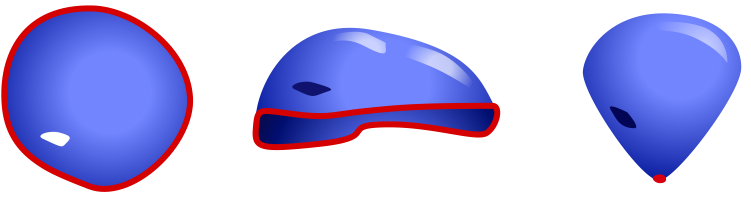
\includegraphics[scale=0.5]{figures/balloons2.png}
    \caption{If there is a gap in the domain that is not a part of the boundary then $\beta_2 = \rank~ \hom_2(\D, \B) = 0$ as there is no void.}
    \label{fig:balloons2}
\end{figure}}

Now suppose our network $P$ covers the domain at some scale $\delta > 0$ such that there are no gaps (1-cycles) in $P^\delta$.
The subset $Q = \B^\delta \cap P$ of points within distance $\delta$ of $\B$ gives us a pair $(P^\delta, Q^\delta)$.
We can verify that the set $P$ covers some subset of the domain by the same process.
A gap in coverage can be through of as ``popping the balloon'' in the sense that, if we wrap the set $P^\delta$ around $Q^\delta$ we would have no void---the gap provides a hole through which the ``air'' can escape, as illustrated in Fig.~\ref{fig:balloons2}.

\subsection{Why short filtrations?}

As we are interested in the coordinate-free setting we will compute the homology of our network using a pair of Rips complexes $\rips_\delta(P, Q) = (\rips_\delta(P),\rips_\delta(Q))$ included into a pair of Rips complexes $\rips_\gamma(P, Q)$.
The reason for this is twofold.

\paragraph{Rips-\v Cech interleaving}

First, the homology of the \v Cech complex can be recovered from this inclusion via the Rips-\v Cech interleaving
\[ \rips_\delta(P, Q) \subseteq \cech_\delta(P, Q)\subseteq \rips_{2\delta}(P,Q).\]
By the nerve theorem this pair of \v Cech complexes is homotopy equivalent to the pair of offsets $(P^\delta, Q^\delta)$ as desired.


\begin{figure}[htbp]
\centering
    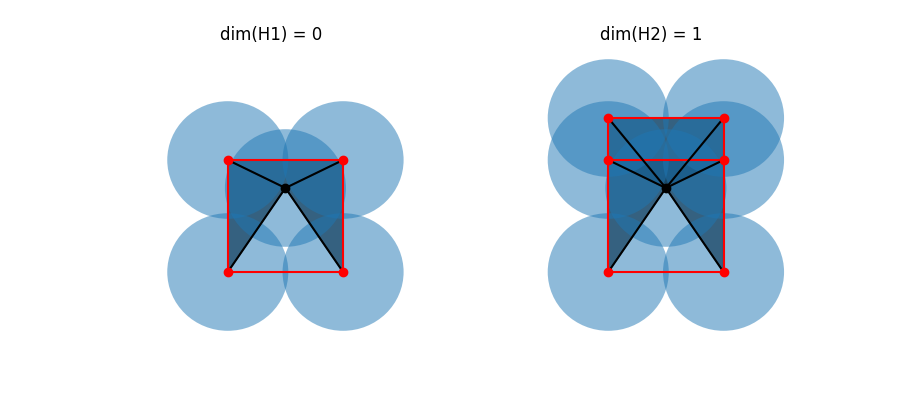
\includegraphics[scale=0.7]{figures/counter.png}
\end{figure}

\paragraph{Fake cycles}
Second, consider a situation in which $P^\delta$ covers $\D$ but there is an additional cycle in $\hom_1(Q^\delta)$ that does not reflect a feature of $\hom_1(\B)$.
In this case there is some point $x\in\D$ surrounded by this cycle that is covered by a point in $P\setminus Q$ but not $Q$.
The result is a non-zero element in $\hom_2(P^\delta, Q^\delta)$ that reflects the void containing this point and not the void corresponding to an element of $\hom_2(\D,\B)$, leading us to a false positive.
Fortunately, this situation is resolved by once again looking at the inclusion $(P^\delta, Q^\delta)\hookrightarrow (P^\gamma, Q^\gamma)$ as any such ``spurious'' cycles are killed for sufficiently large $\gamma > 0$.
This inclusion is contained in the inclusion of Rips complexes $\rips_\delta(P, Q)\hookrightarrow\rips_{2\gamma}(P, Q)$ as follows
\[ \rips_\delta(P, Q) \hookrightarrow \cech_\delta(P,Q)\hookrightarrow\cech_\gamma(P,Q)\hookrightarrow\rips_{2\gamma}(P, Q). \]

\subsection{What do we have? How can we use it?}

The components required to verify a network covers a bounded domain can be summarized by the following
\begin{enumerate}
    \item[a.] the boundary is adequately covered,
    \item[b.] the interior of the domain is covered.
\end{enumerate}
Condition (b) relies on condition (a) in order to provide a topological condition for \emph{coverage} that is necessary but not sufficient.
That is, it can verify coverage alone without false positives but may encounter false negatives.
In fact, the TCC tests a more specific problem: whether we have a reliable representation of the boundary \emph{and} a reliable representation of the interior.

As we have seen, this can be achieved by a collection of sensors that can detect the presence of neighboring sensors at two scales \emph{and} the presence of the boundary.
In reality, it is natural to assume we would like to confirm coverage of a domain in order to measure some quantity.
We therefore consider a situation in which sensors can measure some scalar value, representing a sample of a function defined on the domain.
By defining the boundary in terms of this function we no longer need to require that sensors can detect the presence of the boundary.
Specifically, we can replace the boundary of the domain with a sub-level set that resembles a boundary with specific topological properties.
The points close to the boundary can then be taken as the points measuring function values within a certain range.

In the following section we formalize the notion of a sub-level set resembling a boundary and state the conditions required to confirm coverage.
We then re-state the TCC as a condition that is both necessary \emph{and} sufficient for a more specific problem.% and show how it can be used to approximate the relative persistent homology of the function.
% Finally, we consider classes of functions which satisfy the assumptions made.
% Namely, we consider functions with multiple sub-level sets which may serve as a boundary for this procedure and show how they can be integrated to give a more robust signature for the function.
